\section{Experimental buildup}
%kurz das ziel dieses versuchsteiles ansprechen, damit keine zwei �berschriften direkt �bereinander stehen!
%bei schwierigeren versuchen kann auch der theoretische hintergrund erl�utert werden. (mit formeln, herleitungen und erkl�rungen)
The experimental buildup was developed as part of Staatsexamensarbeit in 1978. A sketch of the buildup can be seen in figure \ref{fig:aufbau}.

The main part of the buildup is the microwave generator, the generator produces waves with a frequency between 18Hz and 27Hz. The waves get directed via a system of waveguides. With an attenuator and a phase shifter the underground signal can be reduced, so the absorption lines are better to see. For measuring the frequency of a peak a wave meter is used, because the resolution of the generator is not high enough. The wave meter uses a cavity, witch drains energy from the system in the case of resonance. For the measurement of the absorption energy is measured with a top diode, witch is connected to a Oscilloscope and a PC for visualization and measuring the signal. The wave guide system is connected with a vacuum pump, to reduce the influence of other gases than the NH3. The amount of NH3 can be controlled with a precision valve.

\begin{figure}[H]
\centering
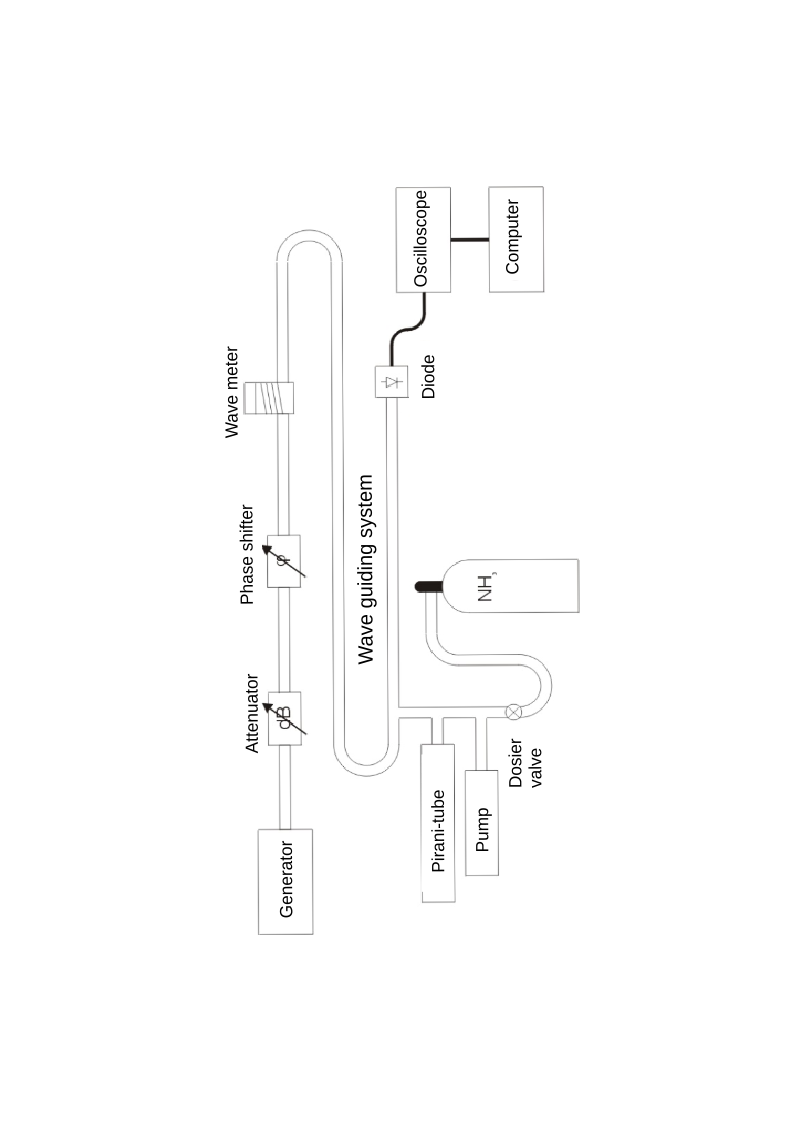
\includegraphics[trim = 50mm 45mm 50mm 45mm, scale = 0.8, angle=-90, clip]{aufbau.png}
\caption{The figure shows the basic buildup of the experiment, the picture was taken from \cite{anleitung} and modified to have English inscriptions}
\label{fig:aufbau}
\end{figure}